\section{Short-Range Correlations - Experiment}
\subsection{Inclusive Measurements}
Inclusive experiments aim to measure precision cross section ratios at $x >$ 1, a region forbidden to the free nucleon.   Electron scattering probes high-momentum nucleons, typically defined as ones with momenta $\ge$300~MeV/c, a few tens of~MeV greater than the Fermi momentum for a given nucleus (there is a range of values, but for $A>12$, most are around 250~MeV/c). If the presence of these high-momentum nuclei is the result of SRCs, then cross sections for A$>$2 will be re-scaled versions of the deuteron cross sections, signaling more SRCs and therefore more high-momentum nucleons in larger nuclei.   A plateau at $x>$1 in the $A/D$ cross-section ratios would support this picture.    Experimentally, in order to obtain enough data points in $x$ to conclusively observe a plateau, there is a threshold Q$^2$ value.  The onset of the scaling plateau moves to lower $x$ values as Q$^2$ increased, but the threshold has typically been taken to be 1.4~GeV$^2$, illustrated with data from Ref.~\cite{Egiyan:2003vg}.

Cross section plateaus at $x>$1 were observed in several JLab experiments~\cite{Egiyan:2003vg, Fomin:2011ng}.  The ratio is proportional to the relative number of high-momentum nucleons in $A$ with respect $D$.  This is not exactly the same as the number of SRC pairs.   The pairs in a $A>2$ nucleus will experience center-of-mass motion due field of the other nucleons.  This will redistribute some strength from the quasielastic peak to the tail of the momentum distribution, resulting in an enhancement in $A>2$ cross sections in the region of interest.  The convention uses $a_2=\sigma_A/\sigma_D$ for raw cross section ratios and $R_{2N}$ for those corrected for the center-of-mass motion of the 2N pair. 


The precision results from JLab E02-019~\cite{Fomin:2011ng} were used to study the nuclear dependence of SRCs. No simple dependence with $A$, density, separation energy or numerous other quantities~\cite{PhysRevC.86.065204} was observed.  However, a deviation of $^9$Be from a simple density dependence analogous to that of the EMC effect was noted.  This led to a number of correlation studies between the two different phenomena and a search for a potential causal effect~\cite{PhysRevC.86.065204, Hen:2012fm, Weinstein:2010rt}.  This is further discussed in Sec.~\ref{sec:SRC_EMC}.

The expectation is to see a second plateau higher in x, in $A/^3\mathrm{He}$ cross section ratios, corresponding to a relative number of 3N configurations in $A$ relative to $^3$He.  Several experiments ~\cite{PhysRevLett.96.082501, Fomin:2011ng, PhysRevC.97.065204}  measured cross sections in the $x>$2 region, but none observed a plateau.  These measurements were done for a range of Q$^2$ values, in order to potentially map out the onset of a 3N plateau, analogously to the case of 2N SRC.  However, defining a kinematic threshold for 3N dominance is more difficult, as there is more than a single configuration that the 3N correlation can take and there are additional dynamics to consider.  One can consider a simple case of a 3N correlation (1-2) where the momentum of one is balanced by two nucleons (rather than a star configuration).  Solving this problem in $\alpha$, which is a light cone analog for $x$, suggests that to see a second plateau over a meaningful $x$ (or $\alpha$) range requires data at higher Q$^2$ values than any of the experiments have previously obtained~\cite{Fomin:2017ydn}.  Collecting adequate statistics for such a result on $^3$He is time prohibitive, and future experiments will more than likely look for the 3N plateau in $A/^4\mathrm{He}$ ratios.  Just as the 2N plateau is seen more cleanly in $A/^3\mathrm{He}$ cross section ratios, a 3N plateau (if it exists) will reveal itself in  $A/^4\mathrm{He}$ ratios, and more cleanly.  There are several reasons that contribute to this, and they include the fact that the cross section in the denominator is going to zero as we approach $x$ of 2 or 3 (for $A/D$ and $A/^3\mathrm{He}$ ratios, respectively) as well as distortion from center-of-mass motion which does not exist in the nucleus in the denominator. 

\subsection{Exclusive Measurements}
A program of exclusive measurements also yielded interesting results. A series of experiments to measure 2N knockout in a kinematic region of large $P_\mathrm{miss}$ that would correspond to a 2N SRC pair revealed that these pairs are predominantly $NP$~\cite{Subedi:2008zz, Shneor:2007tu}.  This observation was consistent with the theoretical calculation~\cite{Schiavilla:2006xx} showing a tensor force dominance in the regime where the first measurements were done and also predicted a weakening of $NP$ dominance with growing $P_\mathrm{miss}$, which follow-up measurements appear to support~\cite{Korover:2014dma}, although with uncertainties that prevent conclusive statements. 


%\subsection{SRC Summary}
%Going into the 12~GeV era at JLab, our future measurements are informed by the following lessons from previous experiments
%\begin{itemize}
%\item Scaling of $A/D$ cross section ratios at $x>$1 observed
%\item No clear nuclear dependence of the $a_2$ ratios
%\item $NP$ dominance of SRC pairs (while significant contributions from FSI are present, they are unlikely to mimic the physics result)
%\item No 3N SRC plateau observed
%\end{itemize}
\section{\label{sec:SRC_EMC}SRC- EMC connection}
When neither SRCs or EMC effect showed a simple nuclear dependence, but both exhibited the same nuclear outliers, several analyses were done to examine the correlation between the two physical phenomena~\cite{PhysRevC.86.065204, Hen:2012fm, Weinstein:2010rt}.  On the surface, it might very well be a coincidence: SRCs are a measure of quasielastic cross sections, whereas the EMC effect probes DIS quark distributions.  Yet, there is room for the two to be related, as the cause for the nuclear modification of structure functions is not understood, and it could come from short-range dynamics probed by SRC measurements.   The other possibility is that both effects arise as the result of the same underlying mechanism rather than having a causal relationship.  Multiple corrections to SRC and EMC measurements were applied to check the robustness of the correlation, but at the end of the, the existing measurements are not precise enough nor span enough nuclei for any meaningful conclusions to be drawn.  Recent work in % FIXME Ref~\cite{} 
proposes a new model for this that consists of a free structure function piece as well as a piece that depends on SRC, and it  reduces the EMC effect to a dependence on the number of protons in the nucleus.  \textit{Wait...is that right}
\begin{figure}[htb]
  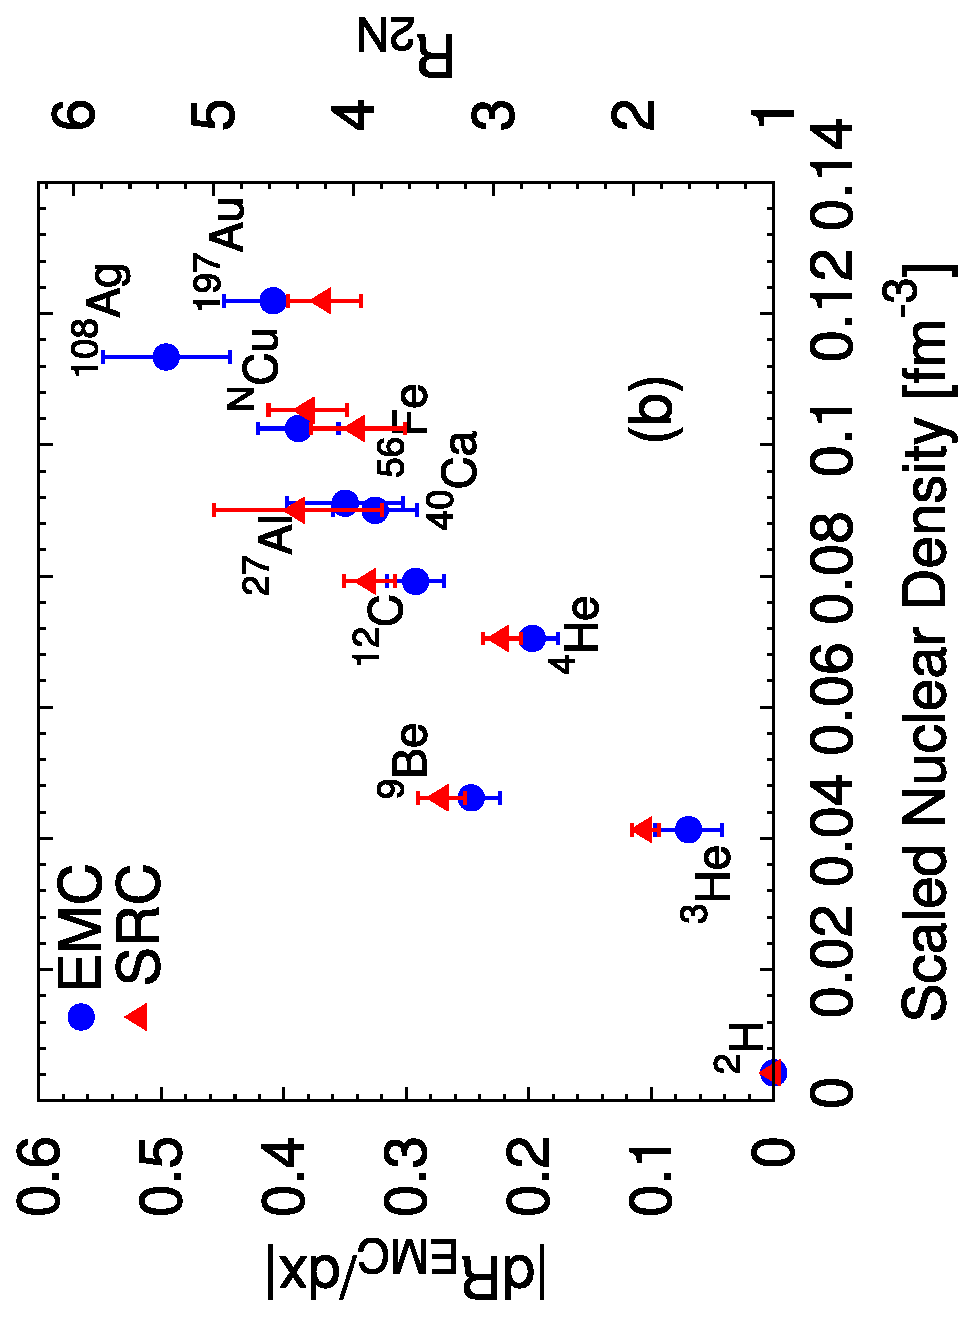
\includegraphics[angle=270, width=0.45\textwidth]{plots/emc_src_vs_scaled_dens_all.eps}
  \caption{Size of the EMC Effect (left axes) as well as the \# of SRC pairs (right axes) as a function of scaled nuclear density}
  \label{fig:src_emc}
\end{figure}
\section{Quarks at $x>$1}
Quasielastic kinematics at $x>$1 probe moving nucleons, but if we increase the Q$^2$, the inelastic contribution begins to dominate, allowing us to access quark distributions. Existing JLab data have a limited range in $x$ and require the application of the of so-called "target-mass corrections" (TMCs) to extract the Q$^2\rightarrow\infty$ structure function limit.  This analysis was done for the E02-019 data, showing that the data are on the edge of... being useful?


